\chapter{Optical Storage Media}
Conventional magnetic data carriers in the form of hard disks or removable disks are traditionally used in computers as secondary storage media. These offer low average access time and provide enough capacity for general computer data at an acceptable price. However, audio and video data, even in compressed form, place heavy demands on available storage capacity. The storage cost for continuous media is thus substantial unless other data carriers are used.

Optical storage media offer higher storage density at a lower cost. The \textit{audio compact disc} (CD) has been commercially successful in the consumer electronics industry as the successor to \textit{long-playing records} (LPs) and is now a mass-produced product.

\section{Basic Technology}
\begin{itemize}
	\item In optical storage media, information is represented by using the intensity of laser light reflected during reading. 
	\item A laser beam having a wave length of about $ 780nm $ can be focused to a resolution of approximately $ 1 \mu m $. 
	\item In a polycarbonate substrate layer, there are depressions, called \textit{pits}, corresponding to the	data to be encoded. 
	\item The areas between the pits are called \textit{lands}.
\end{itemize}

Figure {\ref{fig:cd-pits-lands}} shows a sectional view through an optical disc, running lengthwise along a data track. The pits and lands are represented schematically in the middle of the figure.
%%%%%%%%%%%%%%%%%%%%%%%%%%%%%%%%%%%%%%%%%
%										%
%				FIGURE				   	%
%										%
%%%%%%%%%%%%%%%%%%%%%%%%%%%%%%%%%%%%%%%%%
\begin{figure}[ht!]
	\centering
	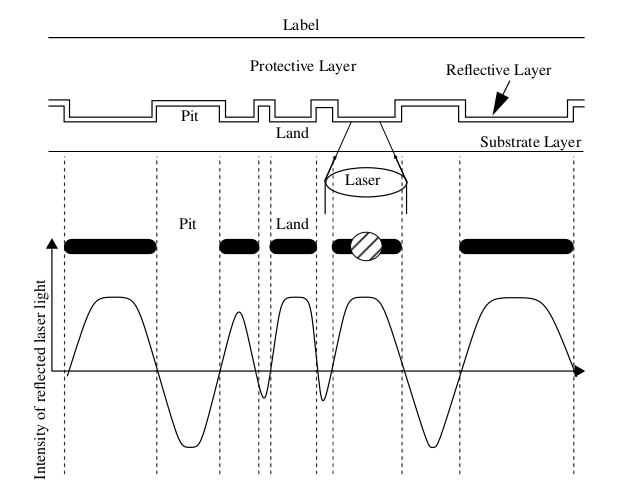
\includegraphics[width=0.8\textwidth]{cd-pits-lands}
	\caption[Sectional view of an optical disc]{Sectional view of an optical disc along the data track. Schematic representation of the layers (top), the ``lands'' and the ``pits'' (middle), and the signal waveform (bottom).}{\label{fig:cd-pits-lands}}
\end{figure}
%--------------------------Figure end -------------------

\begin{itemize}
	\item The substrate layer is smooth and coated with a thin, reflective layer. 
	\item The laser beam is focused at the height of the reflective layer from the substrate level. 
	\item The reflected beam thus has a strong intensity at the lands. 
	\item The pits have a depth of $ 0.12\mu m $ from the substrate surface. 
	\item Laser light hitting pits will be lightly scattered, that is, it will be reflected with weaker intensity. 
	\item The signal waveform shown schematically at the bottom of Figure {\ref{fig:cd-pits-lands}} represents the intensity of the reflected laser light; the horizontal
	line represents a threshold value. 
	\item The laser in the figure is currently sampling a land.
\end{itemize}

According to Figure {\ref{fig:cd-pits-lands}}, a Compact Disc (CD) consists of:
\begin{multicols}{2}
	\begin{itemize}
		\item the label,
		\item the protective layer,
		\item the reflective layer and
		\item the substrate.
	\end{itemize}
\end{multicols}

%%%%%%%%%%%%%%%%%%%%%%%%%%%%%%%%%%%%%%%%%
%										%
%				FIGURE				   	%
%										%
%%%%%%%%%%%%%%%%%%%%%%%%%%%%%%%%%%%%%%%%%
\begin{figure}[ht!]
	\centering
	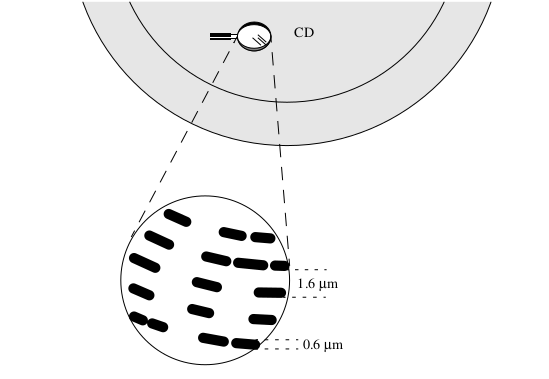
\includegraphics[width=0.7\textwidth]{data-on-cd}
	\caption[Data on a CD as an example of an optical disc]{Data on a CD as an example of an optical disc. Track with ``lands'' and ``pits''.}{\label{fig:data-on-cd}}
\end{figure}
%--------------------------Figure end -------------------

\begin{multicols}{2}
	\begin{itemize}
		\item An optical disc consists of a sequential arrangement of pits and lands within a track. 
		\item The pits and lands represent data on the surface (see Figure {\ref{fig:data-on-cd}}).
		\item All the information on an optical disc is placed on one track. 
		\item The stored information can thus be played back at a continuous data rate
		\item A track is in the form of a spiral. 
		\item In the case of a CD, the spacing between adjacent coils of the spiral—the track pitch is $ 1.6 \mu m$. 
		\item The track width of the pits is $ 0.6 \mu m $, though their lengths can vary. 
	\end{itemize}
\end{multicols}

The light source of the laser can be positioned at a distance of approximately $ 1 mm $ from the disk surface and thus does not touch the disk directly, or float on an air cushion. This reduces wear and tear on the components used and increases the life of the device.

\section{Video Disc Fundamentals}
\begin{itemize}
	\item Video discs in the form of \textit{LaserVision} are used for the reproduction of motion picture and audio data. 
	\item The data are stored on the disc in an analog-coded format, and
	\item the sound and picture quality are excellent. 
	\item \textit{LaserVision} discs have a diameter of approximately $ 30cm $ and store approximately $ 2.6Gbytes $.
\end{itemize}


Motion pictures are frequency-modulated on the video disc, and the audio signal is mixed with the modulated video signal. Figure {\ref{fig:video-disc}} shows the principle used to record data. 
\begin{itemize}
	\item The important information of the mixed audio-video signal is the temporal	sequence of the zero transitions. 
	\item Each zero transition corresponds to a change between a pit and a land on the disc.
	\item Such a change can occur at any time, and is written to the disc in a non-quantized form, that is, the pit length is not quantized. 
	\item This method is thus time-continuous and can be characterized as analog.
\end{itemize}


%%%%%%%%%%%%%%%%%%%%%%%%%%%%%%%%%%%%%%%%%
%										%
%				FIGURE				   	%
%										%
%%%%%%%%%%%%%%%%%%%%%%%%%%%%%%%%%%%%%%%%%
\begin{figure}[ht!]
	\centering
	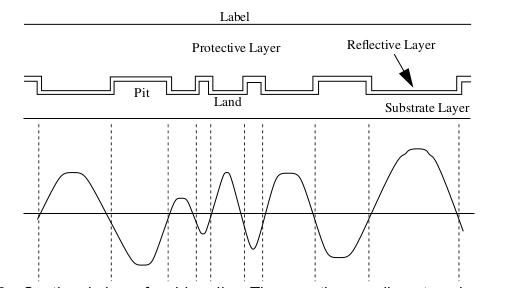
\includegraphics[width=0.8\textwidth]{video-disc}
	\caption[Sectional view of a video disc]{Sectional view of a video disc. Time-continuous discrete value coding.}{\label{fig:video-disc}}
\end{figure}
%--------------------------Figure end -------------------

The video disc was conceived as a Read Only Memory. Since then, many different write-once optical storage systems have come out, known as Write Once Read Many (WORM). An example is the Interactive Video Disc, which operates at Constant Angular Velocity (CAV). On each side, up to 36 minutes of audio and video data at 30 frames per second can be stored and played back. Alternatively, approximately 54,000 studio quality still images can be stored per side.

WORMs have the following special properties:
\begin{itemize}
	\item The term \textit{Media overflow} refers to problems that can occur when a WORM disc is almost full.
	
	\item \textit{Packaging} refers to problems stemming from the fixed block structure of WORMs.
	
	\item \textit{Revision} refers to the problem of subsequently marking areas as invalid.
\end{itemize}

\section{CD Audio, CD ROM and Extended Architecture}
\subsection[CD Audio]{Compact Disc Digital Audio}
The Compact Disc Digital Audio (CD-DA) was developed jointly by N.\ V.\ Philips and the Sony Corporation \textit{for storing audio data}. The basic technology of the CD-DA was developed by N.\ V.\ Philips.

\subsubsection{Technical Basics}
\begin{itemize}
	\item CDs have a diameter of $ 12cm $ and are played at a \textit{Constant Linear Velocity (CLV)}.
	\item The number of rotations per time unit thus depends on the radius of the data currently being sampled. 
	\item The spiral-shaped CD track has approximately 20,000 windings.
\end{itemize}


Information is stored according to the principle depicted in Figure {\ref{fig:cd-pits-lands}} and Figure {\ref{fig:cd-da}}, whereby the length of the pits is always a multiple of $ 0.3 \mu m $. A change from pit to land or from land to pit corresponds to the coding of a $ 1 $ in the data stream. If there is no change, a $ 0 $ is coded.

%%%%%%%%%%%%%%%%%%%%%%%%%%%%%%%%%%%%%%%%%
%										%
%				FIGURE				   	%
%										%
%%%%%%%%%%%%%%%%%%%%%%%%%%%%%%%%%%%%%%%%%
\begin{figure}[ht!]
	\centering
	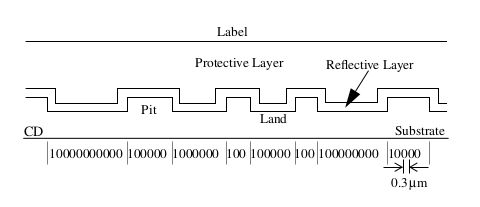
\includegraphics[width=0.8\textwidth]{cd-da}
	\caption[``Pits'' and ``lands'']{``Pits'' and ``lands''. Discrete time, discrete value storage.}{\label{fig:cd-da}}
\end{figure}
%--------------------------Figure end -------------------

\subsubsection{Audio Data Rate}
The audio data rate can easily be derived from the given sampling rate of
$ 44,100Hz $ and the $ 16bit $ linear quantization. The stereo audio signal is pulse code modulated, and the data rate is as follows:
\begin{flalign*}
	& \textrm{Audio data rate}_{CD-DA}\\
	& = 16 \frac{bits}{sample \:value} \times 2 \: channels \times 44,100 \frac{sample \:values}{s \times channel} \\
	& = 14,11,200 \times \frac{bits}{s} \\
	& = 14, 11,200 \times \frac{bits/s}{8 bits /byte} \\ 
	& = 14, 11, 200 \times \frac{\cancel{bits}}{s} \times \frac{byte}{8\cancel{bits}}\\
	& = 14,11,200 \times \frac{byte}{8s}\\
	& = 1,76,400 \times \frac{byte}{s}\\
	& = 176.4\frac{Kbytes}{s} \: \textnormal{(\textnp{१, ७६, ४०० लाई १,००० ले भाग गरेकाे}})  \\
	& \cong  172.3 \frac{Kbytes}{s} \: \textnormal{(\textnp{१, ७६, ४०० लाई १,०२४ ले भाग गरेकाे})} &&
\end{flalign*}
\noindent Where, \textit{$\cong$ means ``is congruent to (that is the equality up to a displacement)"}.\\

Analog long-playing records and casette tapes have a signal-to-noise ratio of
approximately $ 50 $ to $ 60dB $. The quality of the CD-DA is substantially higher. As a rule
of thumb, one can assume $ 6dB $ per bit used during the sampling process. Given $ 16bit $ linear sampling:
\begin{flalign*}
	S/N_{CD-DA} \cong 6\frac{dB}{bit} \times 16 bits  = 96dB
\end{flalign*}
The signal-to-noise ratio is exactly $ 98dB $.

\subsubsection*{Capacity}
The play time of a CD-DA is at least \textit{74 minutes}. Using this value, the capacity of a CD-DA can easily be determined. The capacity given below applies only to storage
used for audio data, without, for example, taking into account data used for error correction:
\begin{flalign*}
    \textrm{Capacity}_{CD-DA} 
    & = 74 min \times 14,11,200 \frac{bits}{s} \\
    & = 74 \times 60 \times 14,11,200 \frac{bits}{s} \\
    & = 6,26,57,28, 000 \frac{bits}{s}\\
   & = 6,26,57,28, 000 bits \times \frac{1}{8\frac{bits}{byte}} \times \frac{1}{1,024\frac{bytes}{Kbyte}} \times \frac{1}{1,024\frac{Kbytes}{Mbyte}} \\
   & \cong 747 Mbytes 
\end{flalign*}

\subsection{CD-ROM}
The Compact Disc Read Only Memory (CD-ROM) was conceived as a storage medium for general computer data, in addition to uncompressed audio data. Further, CD-ROM technology was intended to form the basis for the storage of other media. It was specified by N.\ V.\ Philips and the Sony Corporation in the \textit{Yellow Book} and later accepted as an ECMA standard.

CD-ROM tracks are divided into \textit{audio} (corresponding to CD-DA) and \textit{data} types. Each track may contain exclusively data of one type. A CD-ROM can contain both types of tracks. In a mixed mode disc, the data tracks are usually located at the beginning of the CD-ROM, followed by the audio tracks.

\subsubsection{Blocks}
Since CD-ROMs store general computer data, they require better error correction and higher resolution random access to data units than are specified for CD-DA. A CD-DA has an error rate of $ 10^{-8} $ and allows random access to individual tracks and index points.

This data unit is called a \textit{block}, meaning the \textit{physical block}. In the ISO 9660 standard, there also exists the notion of a \textit{logical block}. The logical block has similar properties to the sectors of other media and file system. 

A CD-ROM block consists of the $ 2,352 bytes $ of a CD-DA block. Thus the $ de facto $ CD-DA standard can serve as the basis for the de facto CD-ROM standard.

Of the $ 2,352 bytes $ of a block, $ 2,048 bytes $ (computer data) or $ 2,336 bytes $ (audio data) are available for user data. The remaining bytes are used for identification for random access and for another error correction layer that further reduces the error rate.

Figure {\ref{fig:cd-rom-data-hierarchy}} shows the data hierarchy of a CD-ROM or CD-DA.

$ 75 blocks $ per second are played back, each consisting of $ 32 frames $. Each frame is
$ 73.5 bytes $ ($ 588 bits $).
\begin{flalign*}
   \textrm{Blocks} &= 14,11, 200 \frac{bits}{s} \times \frac{1}{75}s \times \frac{1}{8bits/byte} \\
   & = 2, 352 bytes 
\end{flalign*}

%cd-rom-data-hierarchy

%%%%%%%%%%%%%%%%%%%%%%%%%%%%%%%%%%%%%%%%%
%										%
%				FIGURE				   	%
%										%
%%%%%%%%%%%%%%%%%%%%%%%%%%%%%%%%%%%%%%%%%
\begin{figure}[hb!]
	\centering
	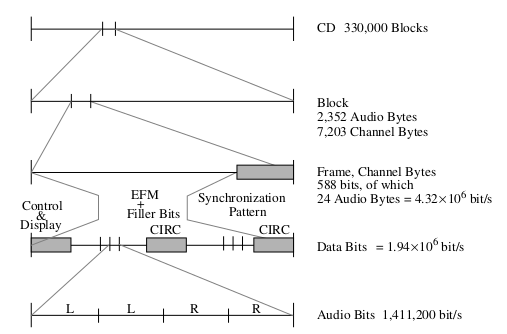
\includegraphics[width=0.8\textwidth]{cd-rom-data-hierarchy}
	\caption[CD-ROM data hierarchy]{CD-ROM data hierarchy. Audio blocks as on a CD-DA}{\label{fig:cd-rom-data-hierarchy}}
\end{figure}
%--------------------------Figure end -------------------

\subsubsection{Modes}
The CD-ROM specification was defined with the goal of storing uncompressed CD-DA data and computer data, as well as serving as the basis for other media. This is
achieved by using two CD-ROM modes:
\begin{multicols}{2}
\begin{itemize}
	\item \textit{mode 1} and
	\item \textit{mode 2}
\end{itemize} 
\end{multicols}


An additional mode $ 0 $, where all $ 2,336 $ user data bytes are set to zero, serves to separate storage areas.

\paragraph*{CD-ROM Mode 1}
\begin{itemize}
	\item CD-ROM mode 1 is used to store computer data, as shown in Figure {\ref{fig:cd-rom-mode-1}}. 
	\item Of the $ 2,352 $ total bytes in each block, $ 2,048 bytes $ are available for storing information.
\end{itemize}

%%%%%%%%%%%%%%%%%%%%%%%%%%%%%%%%%%%%%%%%%
%										%
%				FIGURE				   	%
%										%
%%%%%%%%%%%%%%%%%%%%%%%%%%%%%%%%%%%%%%%%%
\begin{figure}[H]
	\centering
	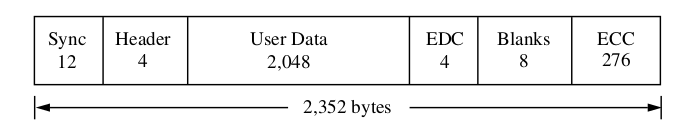
\includegraphics[width=0.8\textwidth]{cd-rom-mode-1}
	\caption[CD-ROM mode 1]{CD-ROM mode 1 block (sector) layout.}{\label{fig:cd-rom-mode-1}}
\end{figure}
%--------------------------Figure end -------------------
To be more exact, the $ 2,352 bytes $ can be broken down into the following groups:

\begin{itemize}
	\item $ 12 bytes $ for synchronization as the start-of-block indicator,
	\item $ 4 bytes $ for the header. This contains an unambiguous block identifier.
	\begin{itemize}
		\item The first	two bytes contain minutes and seconds, respectively; 
		\item the third byte contains the block number, 
		\item while the fourth byte identifies the mode.
	\end{itemize}
	
	\item $ 2,048 bytes $ of user data,
	\item $ 4 bytes $ for error detection,
	\item $ 8 $ unused bytes, and
	\item $ 276 bytes $ for error correction, whereby an error rate of $ 10^{-12} $ can be achieved.
\end{itemize}

A CD-ROM contains $ 3,33,000 blocks $ to be played in$  74 minutes $. The capacity of a CD-ROM with all blocks in \textit{mode 1} can be calculated as follows:

\begin{flalign*}
     {Capacity}_{{CD-ROM}_{Mode \:1}} 
    & = 3,33,000 blocks \times 2, 048 \frac{bytes}{block} \\
    & = 68,19,84,000 bytes \\
    & = 68,19,84,000 bytes \times \frac{1}{1,024 \frac{bytes}{Kbyte}} \times \frac{1}{1,024 \frac{Kbytes}{Mbyte}} \\
    &  \cong 650 Mbytes &
\end{flalign*}

The data rate in \textit{mode 1} is:
\begin{flalign*}
	  {Rate}_{{CD-ROM}_{Mode \:1}}  
     & = 2, 048 \frac{bytes}{block} \times 75 \frac{blocks}{s}\\
     & = 153.6 \frac{Kbytes}{s} \\
     & \cong 150 \frac{Kbytes}{s} 
\end{flalign*}


\paragraph*{CD-ROM Mode 2}
\begin{itemize}
	\item CD-ROM mode 2 serves as the basis for additional specifications for storage of other media.
	\item A block in this mode is shown in Figure {\ref{fig:cd-rom-mode-2}}. 
	\item Of the $ 2,352 $ total bytes in each block, $ 2,336 bytes $ are available for storing information.
\end{itemize}

%%%%%%%%%%%%%%%%%%%%%%%%%%%%%%%%%%%%%%%%%
%										%
%				FIGURE				   	%
%										%
%%%%%%%%%%%%%%%%%%%%%%%%%%%%%%%%%%%%%%%%%
\begin{figure}[H]
	\centering
	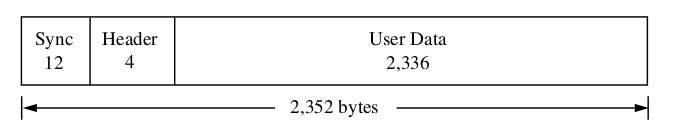
\includegraphics[width=0.8\textwidth]{cd-rom-mode-2}
	\caption[CD-ROM mode 2]{CD-ROM mode 2 block (sector) layout.}{\label{fig:cd-rom-mode-2}}
\end{figure}
%--------------------------Figure end -------------------

The synchronization and header are dealt with as in mode 1. The additional error correction is left out.

The capacity of a CD-ROM with all blocks in mode 2 can be calculated as follows:
\begin{flalign*}
	{Capacity}_{{CD-ROM}_{Mode \:2}} 
	& = 3,33, 000 blocks \times 2,336 \frac{bytes}{block} \\
	& = 77,78,88, 000 bytes \\
	& = 741.8518 Mbytes
\end{flalign*}

The data rate in \textit{mode 2} is:
\begin{flalign*}
	{Rate}_{{CD-ROM}_{Mode \:2}}  
	& = 2,336 \frac{bytes}{block} \times 75 \frac{blocks}{s}\\
	& = 175.2 \frac{Kbytes}{s} \\
\end{flalign*}


\subsection{CD ROM Extended Architecture}
\begin{itemize}
	\item The \textit{Compact Disc Read Only Memory Extended Architecture} (CD-ROM/XA), is based on the CD-ROM specification.
	\item Was established by N.\ V.\ Philips, the Sony Corporation, and Microsoft. 
	\item The main motivation was to address the inadequate consideration paid until then to concurrent output of multiple media.
\end{itemize}


The \textit{Red Book} specifies a track for uncompressed audio data. The \textit{Yellow Book} specifies tracks for computer data using CD-ROM \textit{mode 1} (Figure {\ref{fig:cd-rom-mode-1}}) and tracks for compressed media using CD-ROM \textit{mode 2} (Figure {\ref{fig:cd-rom-mode-2}}).

\begin{itemize}
	\item CD-ROM/XA uses CD-ROM \textit{mode 2} in order to define its own blocks and additionally defines a sub-header that describes each block (sector) as shown in Figure {\ref{fig:cd-xa-form-1}} and Figure {\ref{fig:cd-xa-form-2}}. 
	\item This makes it possible to interleave different media using only \textit{mode 2} blocks, since these can contain different media. 
	\item The individual CD-ROM/XA data	streams are separated during playback.
\end{itemize}





\subsubsection*{Form 1 and Form 2}
CD-ROM/XA differentiates blocks with form 1 and form 2 formats, similar to the CD-ROM modes:

\subsubsection{Form 1}
\begin{itemize}
	\item The XA format form 1 in CD-ROM mode 2 provides improved error detection and correction. 
	\item Like CD-ROM mode 1, 4 bytes are needed for error detection and $ 276 bytes $ for error correction.
	\item Unlike CD-ROM mode 1, the 8 bytes	unused in CD-ROM mode 1 are used for the subheader. 
	\item Figure \ref{fig:cd-xa-form-1} shows a block (sector), where  $2,048 bytes$ are used for data.
\end{itemize}

%%%%%%%%%%%%%%%%%%%%%%%%%%%%%%%%%%%%%%%%%
%										%
%				FIGURE				   	%
%										%
%%%%%%%%%%%%%%%%%%%%%%%%%%%%%%%%%%%%%%%%%
\begin{figure}[ht!]
	\centering
	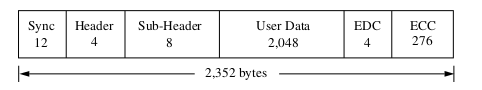
\includegraphics[width=0.8\textwidth]{cd-xa-form-1}
	\caption[Sector layout (1) for CD-ROM/XA according to the ``Green Book''.]{Sector layout (1) for CD-ROM/XA according to the ``Green Book''. Data layout of a CD-ROM block in mode 2, form 1}{\label{fig:cd-xa-form-1}}
\end{figure}
%--------------------------Figure end -------------------


\subsubsection{Form 2}

\begin{itemize}
	\item The XA format form 2 in CD-ROM mode 2 allows a 13 percent increase in actual data capacity, to $ 2,324 bytes $ per block, at the expense of error handling.
	\item Form 2 blocks can be used to store compressed data of various media, including audio and video data.
\end{itemize}

%%%%%%%%%%%%%%%%%%%%%%%%%%%%%%%%%%%%%%%%%
%										%
%				FIGURE				   	%
%										%
%%%%%%%%%%%%%%%%%%%%%%%%%%%%%%%%%%%%%%%%%
\begin{figure}[ht!]
	\centering
	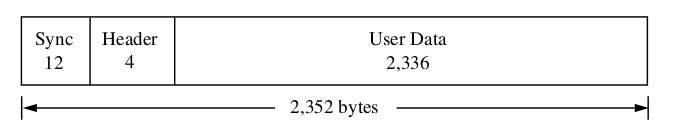
\includegraphics[width=0.8\textwidth]{cd-rom-mode-2}
	\caption[Sector layout (2) for CD-ROM/XA according to the ``Green Book''.]{Sector layout (2) for CD-ROM/XA according to the ``Green Book''. Data layout of a CD-ROM block in mode 2, form 2.}{\label{fig:cd-xa-form-2}}
\end{figure}
%--------------------------Figure end -------------------

\noindent On a CD-DA, CD-ROM, or mixed mode disc, a track always consists of homogeneous data, meaning exclusively audio or computer data. It is thus not possible for the
computer to, for example, concurrently read uncompressed audio data and computer data. 


\subsubsection*{Advantage of CD-ROM/XA}
\begin{itemize}
	\item Blocks of different media can be stored in one track since they are all coded in CD-ROM mode 2.
\end{itemize}

\section{Principles of CD-WO and CD-MO}
\section*{CD Write-Once}
So far, all the CD technologies considered do not allow the user to write to the disk. Thus, the application scope is limited. This has led research laboratories
to develop, besides the \textit{Read Only Storage Media}, compact disks that can be recorded once or several times.

The \textit{Compact Disk Write Once} (CD-WO), like WORM (Write Once Read Many), allows the user to write once to a CD and afterwards to read it many times. CD-WO is specified in the second part of the \textit{Orange Book}.

\subsection{Principle of CD-WO}
Figure {\ref{fig:cd-wo}} shows a cross-section of a CD-WO, vertical to the disk surface and data track. In the case of read-only CDs, the substrate (a polycarbonate) lies directly next to the reflection layer.

%%%%%%%%%%%%%%%%%%%%%%%%%%%%%%%%%%%%%%%%%
%										%
%				FIGURE				   	%
%										%
%%%%%%%%%%%%%%%%%%%%%%%%%%%%%%%%%%%%%%%%%
\begin{figure}[h]
	\centering
	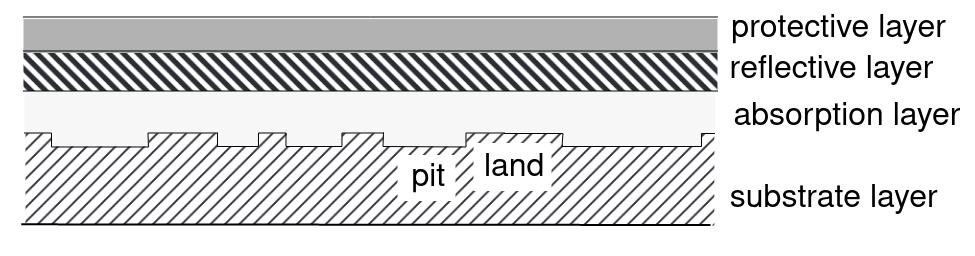
\includegraphics[width=0.8\textwidth]{cd-wo}
	\caption{Cross-section of a CD-WO disc.}\label{fig:cd-wo}
\end{figure}
%--------------------------Figure end -------------------

%\begin{multicols}{2}
\begin{itemize}
	\item In the case of a CD-WO, an \textit{absorption layer} exists between the substrate and the reflection layer. 
	\item This layer can be irreversibly modified through strong thermal influence, which changes the reflection properties	of the laser beams.

		\item In its original state, a CD-WO player recognizes a track consisting of lands. 
		\item The absorption layer in the pre-grooved track is heated to above $ 250 \degree C $ with a laser three to four times the intensity of a reading player. 
		\item Hence, the absorption layer changes such that the reflection of the laser light now corresponds to a pit. 
		\item This method determines the most remarkable property of the CD-WO: its data can be played by any devices which are meant only for read-only CDs.
%\end{multicols}
\end{itemize}

%\subsection*{Sessions}
%\begin{itemize}
%	\item All CD systems described so far assume that a \textit{lead-in area} exists before the actual
%	data area of a CD, and  
%	\item A \textit{lead-out area} exists after the actual data of a CD
%	\item The content is written in a \textit{table of contents} in the lead-in area
%	\item Each player needs this table of contents to position the player correctly
%	\item In the case of writing to a CD-WO, this lead-in area with the table of contents can be
%	overwritten only after the entire write activity is complete
%	\item This means that the actual data of a CD-WO must be written before the table of contents is created
%	\item Therefore, the principle of seueral sessions was introduced, as shown in Figure {\ref{fig:cd-wo-sessions}}
%	\item Bach session has its own lead-in area and lead-out area
%	\item During one write activity, all data for a session are written together with their table of contents, after which the disk can be played on other device
%	\item Thereby the structure of a CD can be extended up to a maximal 99 session
%	\item However, because of the space requirement for lead-in and lead-out areas, at most 46 sessions can be stored
%	\item Each session consists again of its lead-in area, the data area and lead-out area
%	\item Until 1992, all available devices could read only one session
%	\item CD-WOs with only one session are called \textit{regular} CD-WOs. 
%	\item A CD-WO with more than one session is called a \textit{hybrid} CD-WO
%\end{itemize}
%
%
%%%%%%%%%%%%%%%%%%%%%%%%%%%%%%%%%%%%%%%%%%
%%										%
%%				FIGURE				   	%
%%										%
%%%%%%%%%%%%%%%%%%%%%%%%%%%%%%%%%%%%%%%%%%
%\begin{figure}[H]
%	\centering
%	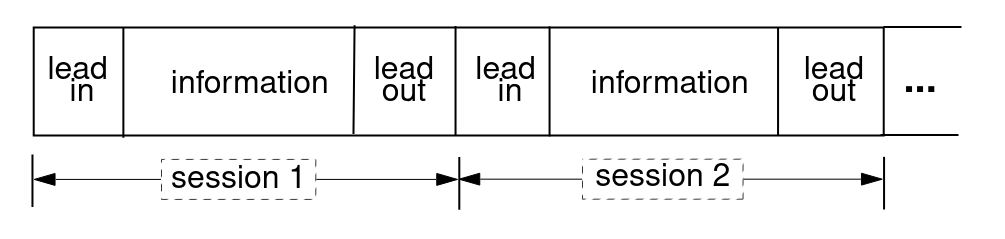
\includegraphics[width=\textwidth]{cd-wo-sessions}
%	\caption{Cross-section of a CD-WO disc}\label{fig:cd-wo-sessions}
%\end{figure}
%%--------------------------Figure end -------------------

\subsection*{CD Magneto Optical}
The Compact Disc Magneto Optical (CD-MO), specified in the first part of the \textit{Orange Book}, has a high storage capacity and allows the CD to be written multiple times.

%%%%%%%%%%%%%%%%%%%%%%%%%%%%%%%%%%%%%%%%%
%										%
%				FIGURE				   	%
%										%
%%%%%%%%%%%%%%%%%%%%%%%%%%%%%%%%%%%%%%%%%
\begin{figure}[ht!]
	\centering
	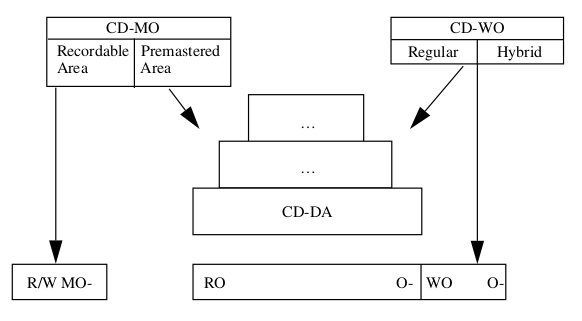
\includegraphics[width=0.8\textwidth]{cd-mo}
	\caption[CD-WO and CD-MO in relation to other CD technologies.]{CD-WO and CD-MO in relation to other CD technologies: structure in multiple layers.}\label{fig:cd-mo}
\end{figure}
%--------------------------Figure end -------------------


\subsection[Principle of CD-MO]{Principle of CD Magnetic-Optical}
\begin{itemize}
	\item The magneto-optical technique is based on the principle that at higher temperatures, a weak magnetic field is needed to polarize the dipoles in certain materials. 
	\item The block (sector) to be written is heated to above $150 \degree C$. 
	\item At the same time, a magnetic field about ten times the strength of the Earth’s magnetic field is applied. 
	\item At this point, the material’s dipoles are polarized towards this magnetic field.
	\item A pit is coded with a downwards-facing magnetic north pole. 
	\item A land is coded using the opposite orientation.
\end{itemize}

In order to erase a block (sector), the area around the block is subjected to a constant magnetic field while it is heated.

If the CD is illuminated by a laser, the polarization of the light changes depending on the magnetization of the CD. In this way, the information can be read.

\subsection*{Areas of a CD-MO}
\begin{itemize}
	\item A CD-MO consists of an optional read-only area and the actual rewritable area.
	\item The read only area (premastered area in Figure {\ref{fig:cd-mo}}) contains data written on the disc in a format specified for this purpose. 
	\item In Figure {\ref{fig:cd-mo}}, this relationship is indicated using the arrows between the premastered area of a CD-MO and the read only technologies. 
	\item Thus, the read only area can be read using existing playback devices.
\end{itemize}

 The rewritable area of a CD-MO cannot be read using existing CD-DA, CD-ROM, CD-ROM/XA, or CD-WO devices due to the fundamentally different technology used for reading and writing. Figure {\ref{fig:cd-mo}} shows the relationships between this recordable area and the underlying magneto-optical technology. This technology is thus incompatible with all the other CD technologies.

\newpage\thispagestyle{empty}